\chapter{Evaluación}
\label{chap:evaluation}
\vspace{0.5cm}

%%%%%%%%%%%%%%%%%%%%%%%%%%%%%%%%%%%%%%%%%%%%%%%%%%%%%%%%%%%%%%%%%%%%%%%%%%%%%%%%
% Objetivo: Exponer los resultados objetivos del sistema                       %
%%%%%%%%%%%%%%%%%%%%%%%%%%%%%%%%%%%%%%%%%%%%%%%%%%%%%%%%%%%%%%%%%%%%%%%%%%%%%%%%

 \lettrine{E}{n} este capítulo exponen los resultados de la evaluación del sistema. Se han seleccionado tres piezas musicales conocidas para realizar las diferentes pruebas. A continuación se describen las tres piezas y las pruebas realizadas. Para realizar una prueba de carga que establezca los límites del sistema se ha añadido una última partitura suficientemente sencilla sobre la que trabajar para poder realizar estas pruebas cómodamente sin preocuparse por la calidad de los resultados.
 
 \begin{itemize}
 	\item \textbf{Menuet:} Famosa pieza de Johann S. Bach, destaca por su simpleza y es interesante para ver como funciona el programa ante compases ternarios. Se sugiere añadir una voz nueva de tesitura más aguda a la presente en la pieza.
 	\item \textbf{Greensleves:} Supuestamente compuesta por Enrique VIII, esta archiconocida partitura presenta una polifonía coral a cuatro voces, ideal para comprobar las capacidades de armonización del sistema. Se sugiere eliminar secciones grandes de la voz solista y ver cómo la completa.
 	\item \textbf{Joy to the World:} Conocido villancico, sería interesante escuchar una reinterpretación de la voz más grave para la pieza, ya sea completando secciones o bien añadiendo una voz de bajo.
 	\item \textbf{The Legend of Zelda:} Tema principal de la conocida saga de videojuegos con el mismo nombre, se ha buscado un arreglo muy sencillo y cercano a la pieza original en 8-bit para poder realizar las pruebas de carga sobre esta pieza.
 \end{itemize}
 
 Para la evaluación se ha empezado por realizar una armonización a compás de cada una de las piezas.
 
 \begin{figure}
 	\centering
 	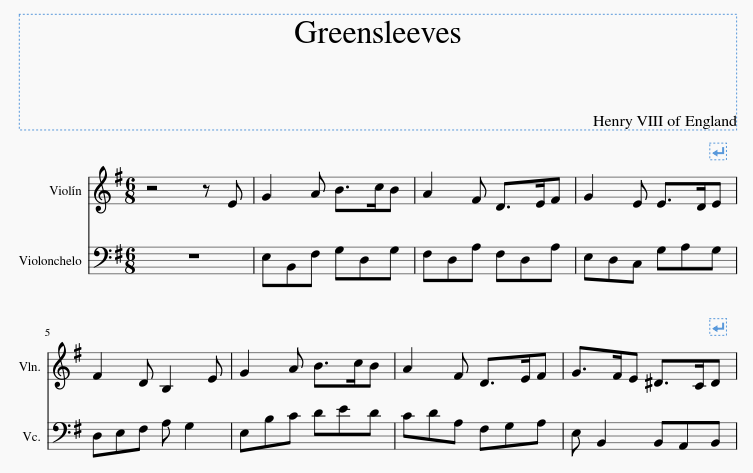
\includegraphics[width=0.8\linewidth]{imagenes/evaluation/greensleeves_orig.png}
 	\caption{Comienzo de Greensleeves sin armonizar}
 	\label{fig:greensleeves_orig}
 \end{figure}
 
  \begin{figure}
  	\centering
  	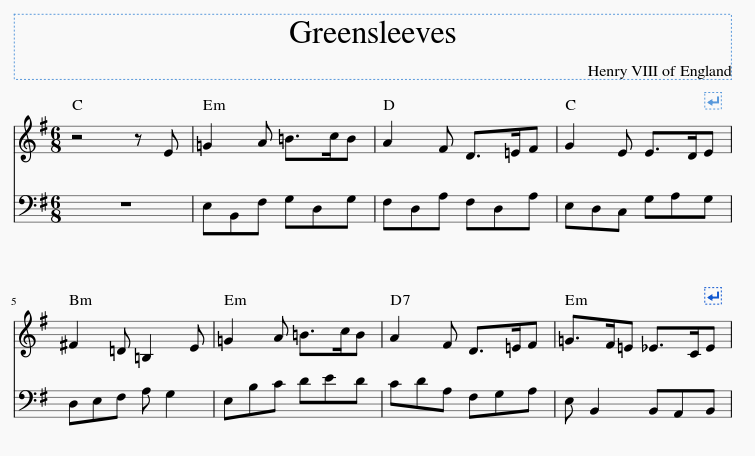
\includegraphics[width=0.8\linewidth]{imagenes/evaluation/greensleeves_harm.png}
  	\caption{Comienzo de Greensleeves armonizado}
  	\label{fig:greensleeves_harm}
  \end{figure}

